\documentclass[12pt]{article}
%Paquetes
\usepackage[left=2cm,right=2cm,top=3cm,bottom=3cm,letterpaper]{geometry}
\usepackage{lmodern}
\usepackage[T1]{fontenc}
\usepackage[utf8]{inputenc}
\usepackage[spanish,activeacute]{babel}
\usepackage{mathtools}
\usepackage{amssymb}
\usepackage{enumerate}
\usepackage{tabularx}
\usepackage{wasysym}
\usepackage{listings}
\usepackage{graphicx}
\usepackage{pmboxdraw}
\usepackage{hyperref}
\usepackage{multicol}
\usepackage{float}
\usepackage[ruled]{algorithm2e}
\renewcommand{\algorithmcfname}{ALGORITHM}
\usepackage{graphicx}
\graphicspath { {media/} }

%Preambulo
\title{Proyecto 2:\\ Implementación de la Optimización por enjambre de particulas para el Problema de la galería de arte }
\author{Carlos Gerardo Acosta Hernández}
\date{Heurísticas de optimización combinatoria 2017-2\\ Facultad de Ciencias UNAM}
\begin{document}
\maketitle
Como segundo proyecto del seminario, decidí implementar el problema de la galería de arte\footnote{} en su
versión con guardias para los vértices de un polígono simple, junto con la heurística de optimización por
enjambre de partículas\footnote{} en su versión binaria para la elección de dichos guardias. En las siguientes secciones abordaré algunos conceptos
importantes para la implementación que realicé, tanto de la heurística, como del problema de mi elección; asimismo, presentaré algunos detalles sobre los componentes de mi sistema, las
entradas y la experimentación a la que lo he sometido hasta el momento. Por último, al final del documento proporciono las instrucciones y herramientas necesarias para construir el sistema y manejarlo con éxito.
\section{Preliminares}
\subsection{Problema de la galería de arte}
El \textit{Problema de la galería de arte} -también conocido como problema del museo-, se puede fácilmente explicar como un problema común en la vida real: Para la disposición de guardias de seguridad en una
galería de arte, encontrar una configuración en la que toda el área de la galería esté resguardada por un número mínimo de guardias. Este problema vio la luz en el año 1973, cuando el matemático estadounidense Victor Klee, inquirió a la comunidad científica sobre cuántos guardias han de ser necesarios para vigilar un polígono de $n$ vértices. Por el momento diremos que un polígono está vigilado si para todo $p \in P$, el segmento de línea formado por
$g \in G$ y $p$ se mantiene \textit{dentro} del polígono, donde $P$ es el conjunto de los puntos en el plano dentro del polígono y $G$ un conjunto de puntos en el plano. En respuesta a la interrogante, Václav Chvátal, propuso propuso y demostró un teorema para este problema en el que se establecía una cota superior de $floor \frac{n}{3}$ del mínimo número de guardias \textbf{necesarios} para vigilar un polígono de $n$ vértices. Es
decir que no siempre es necesario ese número de guardias pero siempre es suficiente. Sin embargo, esta cota sugiere que las soluciones factibles que permanecen cercanas a la suficiencia, siguen estando muy alejadas de
una configuración óptima para los guardias. El problema de hallar tal configuración pertenece a la clase de complejidad \textit{NP-difícil}, incluso para polígonos simples. %cite{}.

Con el fin de definir el problema considerado lo más generalmente posible, es conveniente revisar lo siguiente:
Sea $P$ un polígono con $n$ vertices. Sea $h$ el número de ``hoyos'' en $P$, para este proyecto he decidido trabajar para $h = 0$, es decir que se trabaja con polígonos simples, ya sean convexos o cóncavos.
Para cualesquiera dos puntos $p,q \in V(P)$, el conjunto $V(P)$ de los vértices del póligono, se dice que son ``visibles'' entre ellos si el segmento de recta $pq$ se encuentra ``dentro'' del polígono.
Para definir esta contención en el polígono he considerado estas dos condiciones:
\begin{itemize}
\item Que $pq$ no intersecta ninguna de las aristas del polígono y,
\item el punto medio de $pq$ se encuentra dentro del polígono.  
\end{itemize}
Ahora bien, denotemos el conjunto de visibilidad de un punto $p \in V(P)$ como $M(p) = \{q \in V(P)\;| \;q $ es visible a $p\}$, de manera que para un conjunto de puntos $G \subseteq P$, $M(G)$ estará definido como
$M(G) = \cup_{r \in G} M(r)$. Determinaremos que un conjunto $G \subset V(P)$, vigila a todo el polígono si $M(G) = V(P)$. El objetivo entonces es encontrar un conjunto $G$ vigilante de $P$, tal que su
cardinalidad sea mínima, aquí nos centraremos cuando menos en hallar una cardinalidad que esté por debajo de la cota establecida, de ser posible.





\subsection{Optimización por enjambre de partículas}
La optimización por enjambre de partículas es una heurística inspirada en el comportamiento social colectivo
de agrupaciones o aglomeraciones de seres vivos -manadas, colonias, enjambres, entre otros. Utilizando una población de individuos, el algoritmo tiene por objetivo que cada individuo represente una
solución al problema mediante su posición, codificada en un vector multidimensional del espacio de búsqueda. Además, el individuo debe tener cierta velocidad que le permita actualizar su posición, codificada similarmente en otro vector. La idea general de la búsqueda es que la actualización de la posición de una partícula no sea un mero factor aleatorio, sino que incluya cierta influencia de la mejor solución de toda la población, digamos un individuo destacado que ``lidere'' al colectivo, y la mejor posición que haya encontrado en iteraciones anteriores que no necesariamente es la misma que mantiene en la más reciente. Por tanto, la \textit{exploración} es regida por el factor de aleatoriedad y la \textit{explotación} mediante las posiciones que influyen en la actualización mencionada. De tal suerte que cada partícula tenga posibilidad de explorar con cierta libertad el espacio de búsqueda pero se mantenga cerca del enjambre, que avanza en conjunto hacia valores óptimos.

La heurística, propuesta por Russel Eberhart y James Kennedy en 1995, fue originalmente concebida para espacios de búsqueda contínuos, sin embargo, se han propuesto versiones discretas del algoritmo desde entonces, entre ellas, su versión binaria que implementé para este proyecto. En esta adecuación, cada
entrada en el vector de posición de una partícula es un \textit{bit} y una entrada en el vector
de velocidad representa la probabilidad de que la entrada correspondiente en el vector de posición
se establezca como 1 o 0.

El algoritmo siguiente describe el funcionamiento general de la heurística, por lo que sólo será necesario hacer un par de anotaciones posteriores.

\label{alg:pso}
\begin{algorithm}[H]
  % \SetAlgoNoLine
  \KwIn{n-vertices polygon}
  \KwOut{Best particle in swarm}
  $t \gets 0$;
  $E^t \gets randomValidPopulation(s)$\;
  
  \Repeat{t = maxGen}{
    $t \gets t+1$\;
    \For{each $p_i^t$ in $E^t$}
        {
          \For{each $d = 0,1,...,n-1$}
              {
                $r_p \gets U(0,1)$, $r_g \gets U(0,1)$\\
                $ v_{i,d}^{t+1} \gets \omega v_{i,d}^{t} + \varphi_p r_p (b_{i,d}^{t}-p_{i,d}^t) + \varphi_g r_g (E_{g_d}^t-p_{i,d}^t)$
              }
              update particle's position: $p_{i}^{t+1} \gets p_i^t + v_i^t$
              
              \uIf{$f(p_i^t) < f(b_i^t)$} {
                $b_i^{t+1} \gets p_i^t$
              }
              \uIf{$f(p_i^t) < f(E_g^t)$}{
                $E_g^{t+1} \gets p_i^t$
              }
        }
  }
  \Return $E_g$

  \caption{Particle Swarm Optimization (PSO)}
\end{algorithm}

Aquí vale la pena señalar que $U$ es un generador de números pseudoaleatorios entre [0,1] $\in \mathbb{R}$,
$b_i$ es la mejor posición de la i-ésima partícula del enjambre, $\omega$ es el peso o inercia que
se ejerce sobre la partícula que determina en buena medida su ``movimiento'', $\varphi_p$ y $\varphi_g$ son dos constantes positivas. Estas tres últimas variables, junto con el tamaño $s$ del enjambre o población y el máximo de iteraciones $maxGen$ establecido -que en este caso funge como condición de terminación, pero puede ser sustituido por otro que se considere más conveniente-, son parte de los parámetros que afectan el comportamiento de la heurística y que deben ser explorados durante la experimentaación para mejores (y reproducibles) resultados.\\

Como ya había mencionado, deben hacerse un par de cambios a la versión original, considerando que
por ejemplo, no podemos sumar el vector de posición $p_i \in \{0,1\}^n$ con el vector de velocidad
$v_i \in \mathbb{R}^n$ directamente.
Es por ello, que tanto la actualización de la velocidad como de la posición de la partícula se ven definidos por estas nuevas ecuaciones:
\begin{equation}
  v_{i,d}^{t+1} = \frac{1}{1+e^{-v_{i,d}^t}}
\end{equation}

\begin{equation}
  p_{i,d}^{t+1} =
    \begin{cases*}
      0 & if $r_{i,d} < v_{i,d}^{t}$ \\
      1 & en otro caso
    \end{cases*}
\end{equation}

Donde $r_{i,j} \in \mathbb{R}$ es un número pseudo-aleatorio entre [0,1].

\section{Especificación}
En la presente sección presentaré las herramientas utilizadas para la construcción del sistema, el
diseño utilizado para el código junto con la estrategía general utilizada para la implementación y finalmente algunas de las instancias que se calcularon como entrada de la heurística.

\subsection{Herramientas}
El sistema consta de los siguientes componentes:
\begin{itemize}
\item \textbf{Lenguaje de programación:} Scala 2.12.1
\item \textbf{Sistema de construcción:} SBT (\textit{Scala Build Tool}) 0.13.13
\item \textbf{Documentación:} ScalaDoc 2.12.1
\item \textbf{Pruebas unitarias:} ScalaTest 3.0.1
\item \textbf{Control de versiones:} Para mantener el control de versiones se utilizó Git 2.11.0 y el repositorio en línea se encuentra alojado en GitHub.
\end{itemize}
\subsubsection*{Estructura}\label{sec:e}
El proyecto está organizado con la jerarquía de directorios que se
especifica para proyectos de \textit{SBT} (el sistema de construcción).
El árbol desde el directorio raíz, debe verse como:
\begin{verbatim}
    PSO-AGP/
    ├── build.sbt
    ├── doc/
    ├── instances/
    ├── lib/
    ├── lib_managed/
    ├── project/
    ├── README.md
    └── src/
\end{verbatim}

En la carpeta \textbf{doc}/, se encuentra este documento que estás
leyendo, y su código fuente en \LaTeX. \\

En la carpeta de \textbf{lib}/, se incluyen las bibliotecas externas al sistma de
construcción y al lenguaje de programación de las que depende el
proyecto. Para este proyecto en particular tenía contemplado utilizar \textit{JavaFX} o en su
defecto \textit{ScalaFX} para una interfaz gráfica interactiva, sin embargo aún no hay implementación lista para tal propósito.\\

En el directorio \textbf{instances}/, se encuentran las instancias de entrada del sistema. Archivos
con terminación $.pol$, en referencia a la palabra polígono y un subdirectorio \textbf{solutions}/,
con imágenes en formato $SVG$ producidas al termino de cada ejecución, que deben poseer el mismo
nombre que la instancia de la que provienen. Presentaré el formato de las instancias en la última
sección que corresponde a la experimentación con dichos archivos (Sección \ref{sec:m}).\\

Todo el código fuente referido a la implementación de la heurística
se encuentr en el directorio \textbf{src}/. Desde ahí es posible exploar
el código. Es importante recalcar que se incluye una carpeta para código
escrito en \textit{Java}, sin embargo, se encontrará vacía, pues la
implementación está realizada por completo con la sintáxis de \textit{Scala}. Hay dos subdirectorios en dicha sección, pero lo retomaremos más
adelante en diseño (Sección \ref{sec:c}).\\

En \textbf{project} están definidas las dependencias del proyecto en un
archivo de nombre \textbf{Dependencies.scala}, donde se definen las características del sistema de construcción (puede señalarse, por ejemplo, una versión específica de \textit{SBT} que será descargada en cuanto se inicialice el proyecto por la versión actual que tenga el sistema). Asimismo pueden agregarse todas las dependencias que sean necesarias, por el momento sólo se define la de \textit{ScalaTest} para pruebas unitarias.\\


\subsection{Diseño}\label{sec:c}
Como se mencionaba en la sección anterior, la implementación está dividida en dos paquetes principales, subdirectorios del paquete raíz de código fuente de \textit{Scala}.
\begin{verbatim}
    src/main/scala/
    ├── AGP/
    ├── BPSO/
    ├── Controlador.scala
    ├── Main.scala
    └── SVG.scala
\end{verbatim}

El paquete \textbf{AGP} contiene todo los referente al modelado de polígonos, mientras que \textbf{BPSO}\footnote{Se refiere a \textit{Binary Particle Swarm Optimization}} contiene todas las implementaciones necesarias para la heurística.
A diferencia del proyecto 1, he decidido no hacer \textit{traits} previo al modelado, pues resultaban
altamente dependientes del problema, por lo que una modularización para cada componente de la heurística me pareció suficiente. Aunque claro, conserva cierto parecido con la diligencia de ese primer proyecto.

\begin{multicols}{2}
\begin{enumerate}
\item CTerminacion.scala
\item FuncionDeCosto.scala
\item GeneradorVerificador.scala
\item Enjambre.scala
\item BPSO.scala
\item Particula.scala

\item Poligono.scala
\item Punto.scala
\end{enumerate}
\end{multicols}

Al respecto de los archivos libres en la carpeta, como su nombre indica \textit{Controlador.scala}
es el código encargado de iniciar la ejecución de la heurística con la entrada provista, \textit{Main.scala} es el código encargado de la interfaz de usuario para el uso del sistema y \textit{SVG.scala}
una herramienta de dibujo para las instancias (los polígonos). 
Para información más detallada de la implementación, favor de revisar
\textit{target/scala-2.12/api/}\textbf{index.html} con la \textit{API} generada por \textit{ScalaDoc}.

\subsection{Función de costo}
\subsection{Experimentacion}\label{sec:m} %instancias
\subsubsection*{Archivo de configuración}
Dentro de la carpeta de \textbf{instances}/ he incluído algunas de las instancias que probé para el sistema, ya con el formato requerido para la interfaz de usuario. Todo archivo de entrada debe contar
en su primera línea con 6 argumentos separados por comas y \underline{sin espacios}, en el siguiente orden
\begin{enumerate}
\item La semilla para el generador de números pseudoaleatorios
\item El tamaño del enjambre, i.e., el número de partículas de la población
\item El máximo número de iteraciones
\item $\omega$, el peso o la inercia constante que se ejerce sobre las partículas
\item $\varphi_p$, el factor de influencia de la mejor posición de la partícula
\item $\varphi_g$, el factor de influencia de la posición de la mejor partícula en el enjambre
\end{enumerate}
Es decir que la primera línea debe tener la siguiente sintáxis:
\begin{verbatim}
[semilla],[tamaño_enjambre],[max_iter],[omega],[phi],[phi2]
\end{verbatim}

Las siguientes líneas deben corresponder a un vértice del polígono, siendo cada i-ésimo punto adyacente con
el (i+1)-ésimo, por supuesto módulo n, es decir que el primero es adyacente con el último.
Cada vértice debe constar de una coordenada $x$ y una coordenada $y$ en $(x,y) \in \mathbb{R}^2$,
separadas por una coma y sin espacios, sin parentesis ni nada más que un salto de línea luego de la $y$. 

\begin{verbatim}
                      x,y
                      x2,y2
                      x3,y3
                      ...
\end{verbatim}


A continuación se encuentran algunos ejemplos de las instancias más relevantes con los parámetros
para hallar la mejor solución hasta el momento del sistema.
\begin{multicols}{2}
\begin{figure}[H]
  \centering
  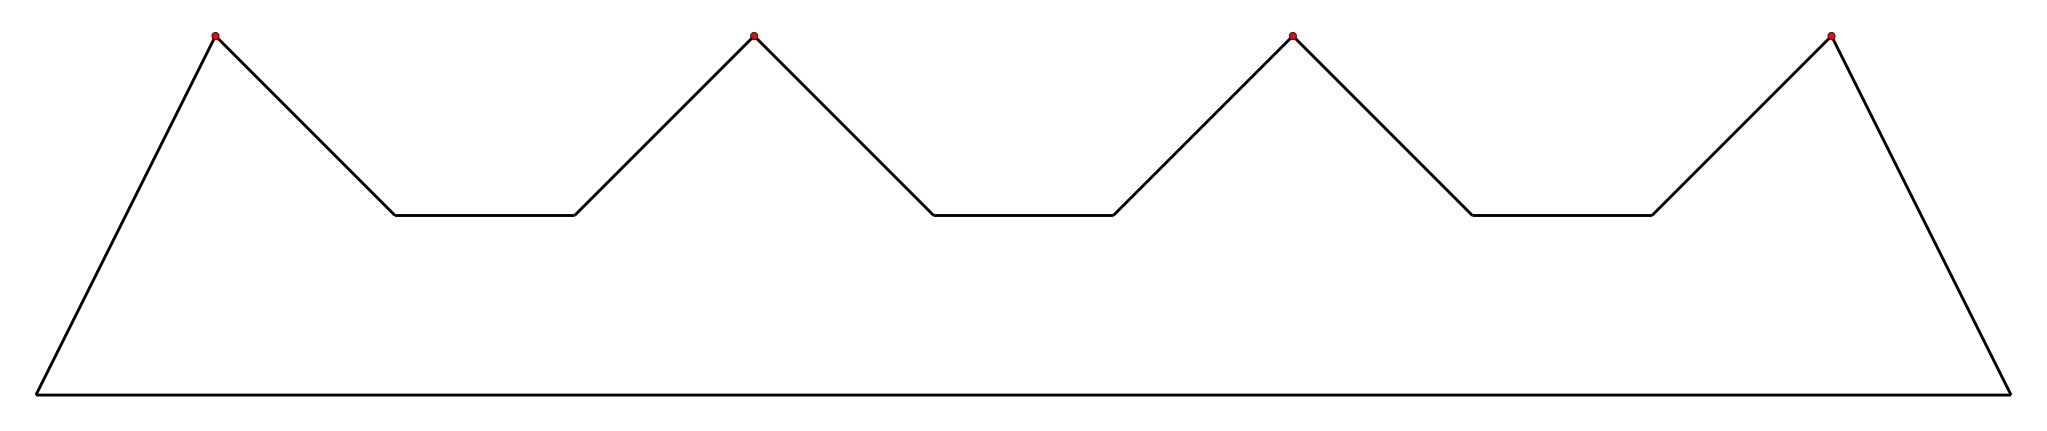
\includegraphics[width=.5\textwidth]{peine}
  \caption{Solución factible a instancia \textit{peine.pol}.}
\end{figure}
\texttt{
\begin{enumerate}
\item Semilla = 1
\item Tamaño del enjambre = 100
\item Máximo de iteraciones = 100
\item $\omega$ = , $\varphi_p$ = ,$\varphi_g$ = 0.1, 0.1, 0.1
\end{enumerate}
}
\end{multicols}

\begin{multicols}{2}

\begin{figure}[H]
  \centering
  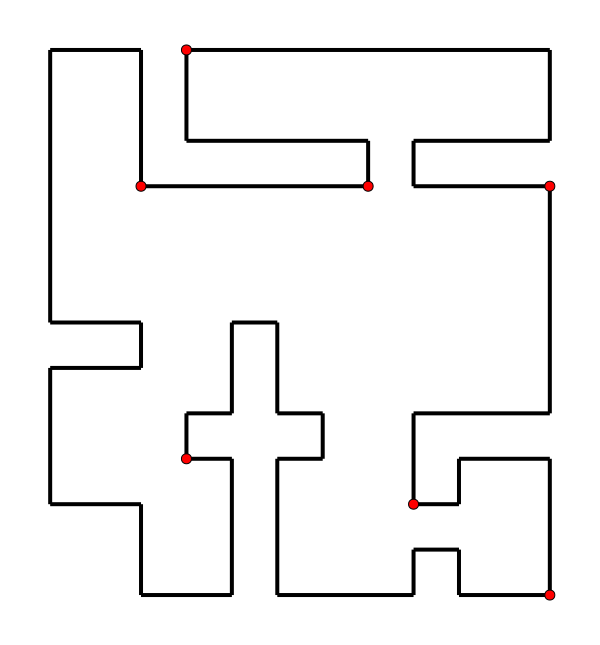
\includegraphics[width=.3\textwidth]{galeria}
  \caption{Solución factible a instancia \textit{galeria.pol}.}
\end{figure}
\texttt{
\begin{enumerate}
\item Semilla = 23
\item Tamaño del enjambre = 2000
\item Máximo de iteraciones = 100
\item $\omega$ = -1.5, $\varphi_p$ = 0.0003,$\varphi_g$ = 0.004 
\end{enumerate}
}
\end{multicols}

\begin{multicols}{2}
\begin{figure}[H]
  \centering
  \includegraphics[width=.4\textwidth]{edificio}
  \caption{Solución factible a instancia \textit{StSerninH.pol}.}
\end{figure}
\texttt{
\begin{enumerate}
\item Semilla = 1
\item Tamaño del enjambre = 10000
\item Máximo de iteraciones = 100
\item $\omega$ = -1.2, $\varphi_p$ = 0.0001 ,$\varphi_g$ = 0.01
\end{enumerate}
}
\end{multicols}

\section{Manejo del sistema} %compilacion y ejecucion
\subsubsection*{Descarga del proyecto}
El proyecto se encuetntra alojado en línea en \textit{GitHub}, para
descargarlo basta ejecutar \textit{Git} en cualquier directorio del
sistema de archivos.
\begin{verbatim}
    $ git clone https://github.com/Pernath/PSO-AGP.git
\end{verbatim}
Se creará un directorio con la estructura definida en la sección \ref{sec:c}.
\subsubsection*{Compilación y ejecución}
Para las operaciones siguientes se supone que el sistema operativo ya cuenta con el sistema de construcción \textit{sbt} instalado.\\

\noindent
En primer lugar llamamos al sistema de construcción, que buscará el
archivo \textbf{build.sbt} y establecerá la ruta actual como la ruta
del proyecto.
\begin{verbatim}
    [user@host PSO-AGP]$ sbt
\end{verbatim}
Esto nos llevará a un \textit{prompt} desde el que podremos llamar
los siguientes comandos de acuerdo a lo que necesitemos.

Para compilar el proyecto y verificar que todo está listo.
\begin{verbatim}
    > compile
\end{verbatim}
Posteriormente, será posible ejecutar el programa con el archivo de configuración como argumento.
\begin{verbatim}
    > run conf.txt
\end{verbatim}
Este archivo debe cumplir el formato especificado en \ref{sec:m}.
\subsubsection*{Empaquetado}
Una manera de empacar la implementación es ejecutar el siguiente comando:
\begin{verbatim}
    > package
\end{verbatim}
Sin embargo, este no incluirá las dependencias externas en el \textit{JAR} generado bajo la ruta \textit{target/scala-2.12/}\textbf{AGP.jar}, por lo que no será portátil y dependerá \underline{siempre} de la estructura de directorios del sistema.

Por fortuna, también incluí la opción para generar un \textit{stand-alone JAR} que nos permitirá mover líbremente el ejecutable de \textit{Java} y ejecutarlo desde cualquier directorio. Esto se logra con el
siguiente comando y podrá encontrarse el ejecutable en la misma dirección mencionada anteriormente:
\begin{verbatim}
    > assembly
\end{verbatim}
Este también ejecutará las pruebas unitarias incluídas en \textbf{src/test/}.

\subsubsection*{JAR}
Para ejecutar el resultado del ensamblaje, debemos ubicar el archivo \textit{JAR} en la carpeta mencionada.
\begin{verbatim}
    [user@host scala-1.12]$ java -jar AUTSP.jar conf.txt
\end{verbatim}
Es importante recordar que este paquete será bastante más rápido en ejecución que realizando un \textit{run} sobre el ``prompt'' de $sbt$.
\end{document}
